\PassOptionsToPackage{table}{xcolor}
\documentclass[aspectratio=169]{beamer}\usepackage[utf8]{inputenc}
\usepackage{lmodern}
\usepackage[english]{babel}
\usepackage{color}
\usepackage{amsmath,mathtools}
\usepackage{booktabs}
\usepackage{mathptmx}
\usepackage[11pt]{moresize}
\usepackage{hyperref}
\usepackage{commath}
\usepackage{bm}
\usepackage{subfigure}
\usepackage{siunitx}

\setbeamertemplate{navigation symbols}{}
\setbeamersize{text margin left=5mm,text margin right=5mm}
\setbeamertemplate{caption}[numbered]
\addtobeamertemplate{navigation symbols}{}{
\usebeamerfont{footline}
\usebeamercolor[fg]{footline}
\hspace{1em}
\insertframenumber/\inserttotalframenumber}

\newcommand{\R}{\mathbb{R}}
\newcommand{\E}{\mathbb{E}}
\newcommand{\N}{\mathbb{N}}
\newcommand{\Z}{\mathbb{Z}}
\newcommand{\V}{\mathbb{V}}
\newcommand{\Q}{\mathbb{Q}}
\newcommand{\K}{\mathbb{K}}
\newcommand{\C}{\mathbb{C}}
\newcommand{\T}{\mathbb{T}}
\newcommand{\I}{\mathbb{I}}
\DeclareMathOperator{\sign}{sign}

\title{Time delta ($\delta$)}
\subtitle{Renzo Miguel Caballero Rosas}

\begin{document}

\begin{frame}
\titlepage
{\tiny Note: We compute the following results using \textbf{initial\_time.m}.}
\end{frame}


%\setbeamercolor{background canvas}{bg=white!10}
%\begin{frame}\frametitle{Extra: Interesting data processing}
%
%\begin{figure}[ht!]
%\centering
%\includegraphics[width=0.4\textwidth]{../../../Python/Represas_Data_2/Wind_Data/someResults/final/mean_error.eps}\quad\quad
%\includegraphics[width=0.4\textwidth]{../../../Python/Represas_Data_2/Wind_Data/someResults/final/mean_abs_error.eps}
%\end{figure}
%{\small What we are seeing is the \textbf{mean error} and \textbf{mean absolute error} as a function of the forecast. This is, for each interval with length 0.1 (i.e., [0,0.1), [0.1,0.2), etc.), we average all the errors corresponding to measurement where the forecast was in that intervals, and after we average over the number of elements in each interval. \alert{In some future, we can use this information to construct an even more realistic model.}}
%
%\end{frame}


\setbeamercolor{background canvas}{bg=white!10}
\begin{frame}\frametitle{\alert{\textbf{Copied from the paper (19/03/20):}}}

We can estimate $\delta$ solving the problem

\begin{equation*}
\delta\approx\arg\min_{\delta}\mathcal{L}_{\delta}(\bm{\theta},\delta; V^{M,1}) = \arg\min_{\delta}\prod\limits_{j=1}^M \rho_0 (V_{j, t_0}|V_{j, t_{-\delta}};\bm{\theta},\delta).
\end{equation*}

\end{frame}


\setbeamercolor{background canvas}{bg=white!10}
\begin{frame}\frametitle{\alert{\textbf{Copied from MATLAB's slides (19/03/20):}}}

We have that, for almost all days, at time $t=t_0$, $X(t_0)\neq p(t_0)$ and then $V(t_0)\neq0$. However, by forecast construction, there should exist a time $t_{-\delta}<t_0$ such that $V(t_{-\delta})=0$.\\
\quad\\
We extrapolate linearly $p(t)$ so we can evaluate $p(t_{-\delta})$, and assume that $V(t_{-\delta})=0$. Then, for each day $j$, we have an initial transition $(V_{j, t_0}|V_{j, t_{-\delta}};\bm{\theta},\delta)$. We assume again that it is Beta and apply the same moment matching as for the rest of transitions. With our initial guess for $\bm{\theta}$, we can construct our initial guess for $\delta$ solving the problem

\begin{equation*}
\delta\approx\arg\min_{\delta}\mathcal{L}_{\delta}(\bm{\theta},\delta; V^{M,1}) = \arg\min_{\delta}\prod\limits_{j=1}^M \rho_0 (V_{j, t_0}|V_{j, t_{-\delta}};\bm{\theta},\delta) \,.
\label{likelihood_delta}
\end{equation*}

\alert{We got $\delta\approx\SI{80}{\min}$.}

\end{frame}


\setbeamercolor{background canvas}{bg=white!10}
\begin{frame}\frametitle{Step by step: (WLOG we can use $t_0=0$ and $t_{-\delta}=-\delta$)}

We are imposing that $V_{j,t_{-\delta}}=0$ for all $j\in\{1,\dots,M\}$, there $t_{-\delta}=t_0-\delta$. Then, for each path $j$, we have that the first moment $m_1(t)=0$ for all $t\in[t_{-\delta},t_0]$.\\
\quad\\
The second moment is given by
\begin{equation}
\begin{cases}
\frac{\dif m_2}{\dif t}&=-\underbrace{2\theta_t(1+\alpha)}_{k_1(t)}m_2+\underbrace{2\theta_t\alpha}_{k_2(t)} \underbrace{p_t(1-p_t)}_{f(t)}\\
m_2(t_{-\delta})&=0.
\end{cases}
\label{S1}
\end{equation}
Then, as $m_1(t_0)=0$, the R.V. $V_{j,t_0}|(V_{j,t_{del
}}=0)$ can be extracted from
\begin{equation*}
2\times\text{Beta}\left(\frac{1-m_2(t_0)}{2m_2(t_0)},\frac{1-m_2(t_0)}{2m_2(t_0)}\right)-1,
\end{equation*}
which has mean and variance
\begin{equation*}
\mu=0,\quad\sigma^2=m_2(t_0).
\end{equation*}

\end{frame}


\setbeamercolor{background canvas}{bg=white!10}
\begin{frame}\frametitle{Step by step:}

If we assume that $\theta_t=\theta_0$ in $[t_{-\delta},t_0]$, the system (\ref{S1}) has solution
\begin{equation*}
m_2({t})=e^{-k_1{t}}\int_{t_{-\delta}}^{{t}}k_2e^{k_1s}f(s)\dif s.
\end{equation*}
As $p_t(1-p_t)\leq1/4$ in $[t_{-\delta},t_0]$, we have the bound
\begin{equation*}
m_2({t})\leq\frac{\frac{k_2}{4}\int_{t_{-\delta}}^{{t}}e^{k_1s}\dif s}{e^{k_1{t}}}=\frac{k_2}{4k_1}\left(1-\frac{e^{k_1t_{-\delta}}}{e^{k_1{t}}}\right)\leq\frac{1}{4}\left(1-e^{k_1(t_{-\delta}-t)}\right).
\end{equation*}
Then, $\lim_{t_{-\delta}\to-\infty}m_2(t_0)\leq 1/4\implies\sigma^2\leq1/4$.\\
\quad\\
{\footnotesize
Then, if we need more variance to model the initial transition, we can not use this model. Noticed that we assumed $\theta_t=\theta_0$ in $[t_{-\delta},t_0]$, this is not true in general as $p_{t_{-\delta}}$ can be very near the boundaries $\epsilon$ and $1-\epsilon$. However, even with the assumption, to have limit variance is a problem as for some set of data the assumption can hold. Still, if the initial error is so large, we would not be able to model it correctly with limited variance.}
\end{frame}


\setbeamercolor{background canvas}{bg=white!10}
\begin{frame}\frametitle{Step by step: We remove points with $|V_{j,t_0}|>\eta=0.1$}

\begin{figure}[ht!]
\centering
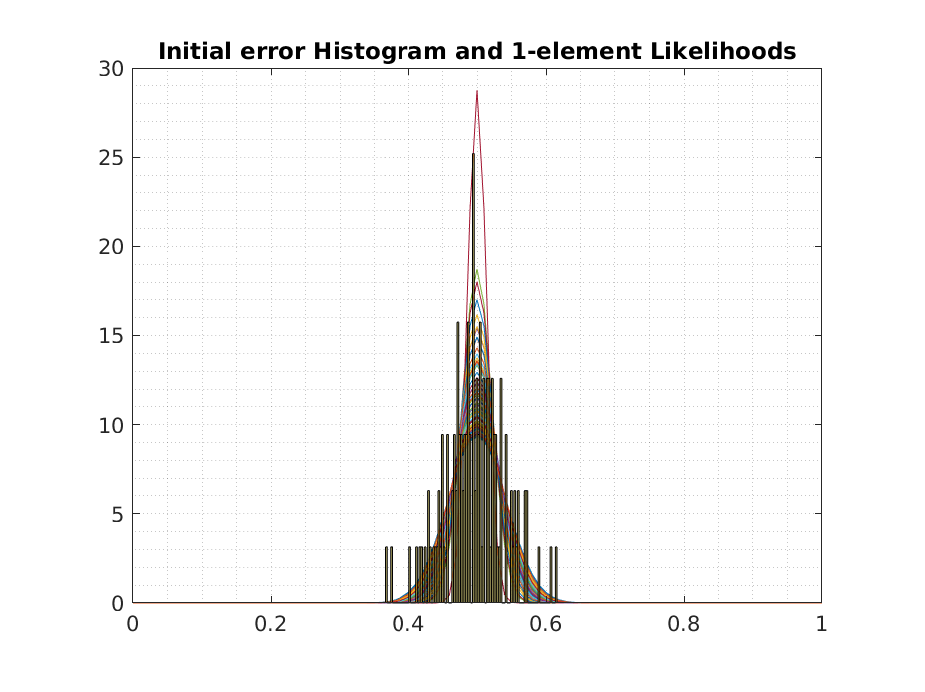
\includegraphics[width=0.45\textwidth]{../../MATLAB_Files/Results/delta/allLH_0.eps}
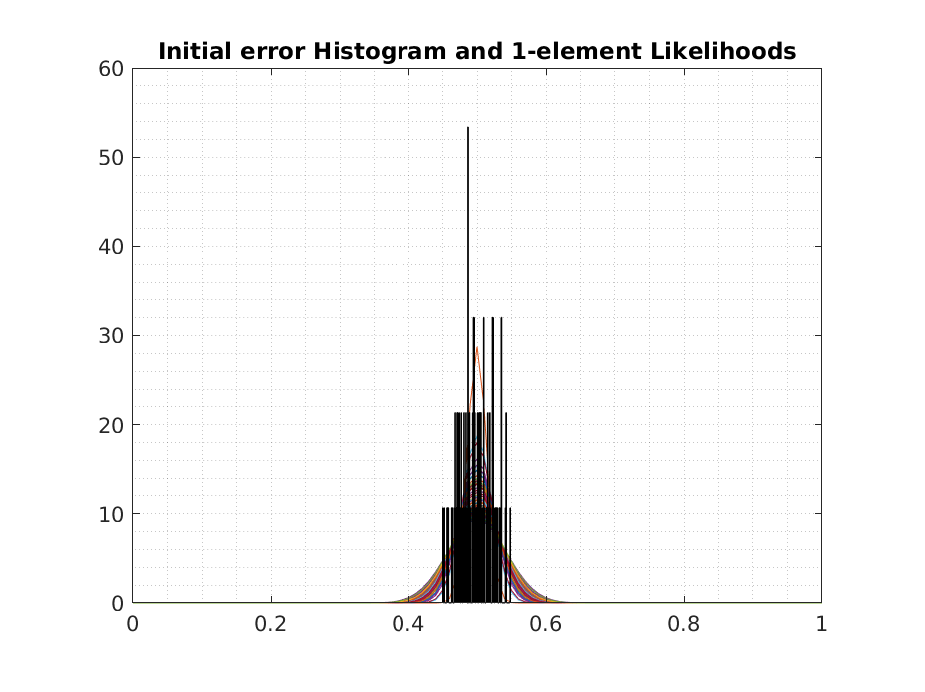
\includegraphics[width=0.45\textwidth]{../../MATLAB_Files/Results/delta/allLH_1.eps}
\end{figure}
{\small
Here we can see all the likelihoods for each initial transition when $\delta=\text{*one day*}$, overlapped with histograms of the initial error. On the left, we use all the initial errors, and clearly, the distribution that fits that histogram needs more variance. On the right, we removed the points with more error, and we can see that we need $\delta<\text{*one day*}$.}
\end{frame}


\setbeamercolor{background canvas}{bg=white!10}
\begin{frame}\frametitle{Step by step: Explanation Problem-Solution}

Basically, what happens is that the variance in the initial point grows with $\delta$ (the more in the past we *start*, the more variance we have at time $t=0$ or $t_0$).\\
\quad\\
The problem is that, as $\delta\uparrow$, we have that $m_2(t_0)\uparrow$. At the same time, as $m_1(t)=0$ (because we fix $V_{j,t_{-\delta}}=0$ for all $j\in\{1,\dots,M\}$), we can prove that $m_2(t_0)\leq1/4$ for all possible $\delta>0$.\\
\quad\\
Now, we have that $\xi_1=\xi_2$ in the Beta distribution, and then $\sigma^2=m_2(t_0)$ for the distribution of $V_{j,t_{-\delta}}$. Then, the variance is bounded by 1/4. This means that, if the set of errors at the initial time has a larger variance, we will not be able to reach the correct Beta distribution using the moments matching.\\
\quad\\
How we solve this problem? Two options: Change model to one with more possible variance, or remove the data with substantial error. {\color{orange}We remove all data s.t. $|V_{j,t_0}|>\eta$ for some $\eta>0$.} To create this new dataset we use \textbf{new\_batch\_fixed\_removed\_samples.m}.

\end{frame}


\setbeamercolor{background canvas}{bg=white!10}
\begin{frame}\frametitle{Step by step:}

\begin{figure}[ht!]
\centering
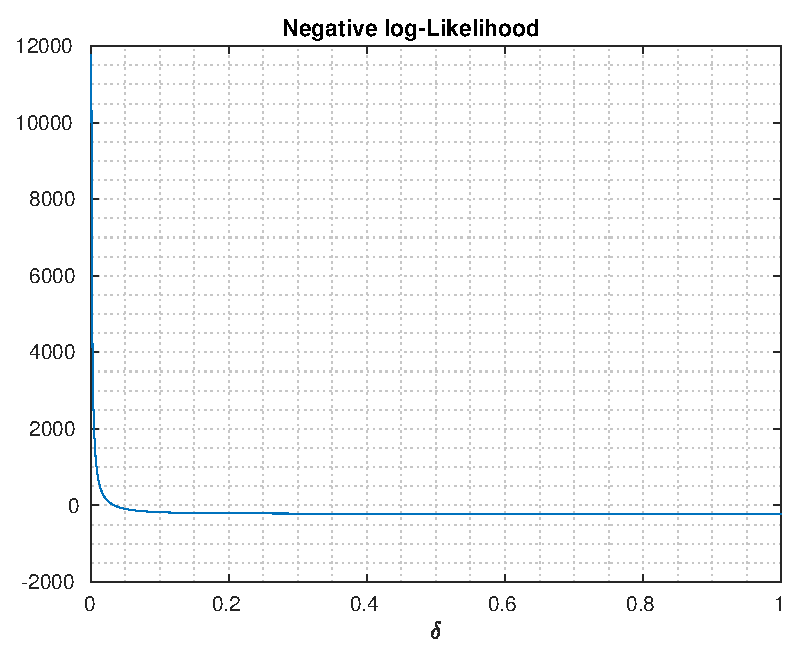
\includegraphics[width=0.45\textwidth]{../../MATLAB_Files/Results/delta/LL_0.eps}
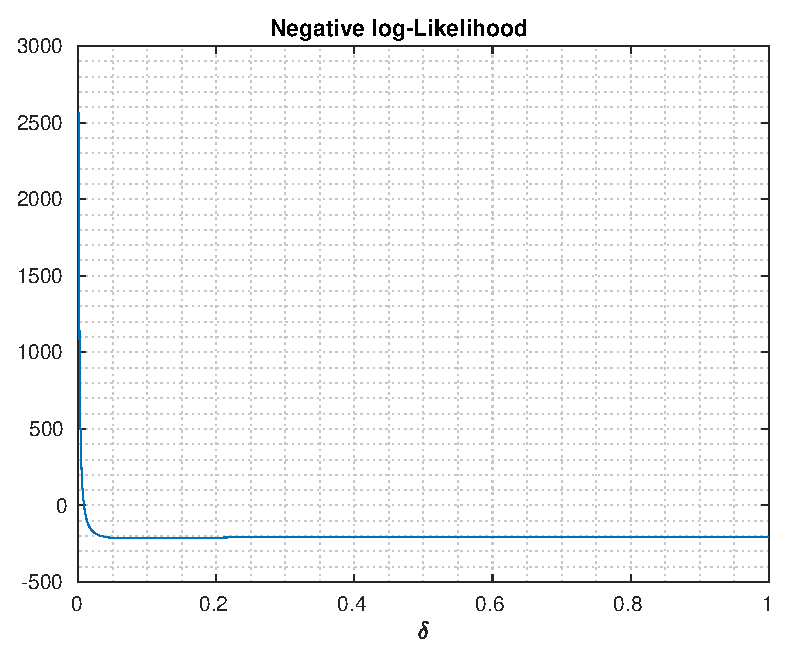
\includegraphics[width=0.45\textwidth]{../../MATLAB_Files/Results/delta/LL_1.eps}
\end{figure}
On the left, negative log-likelihood using all the data. On the right, using only the {\color{orange}*corrected data* with $\eta=0.1$}. In the next slide we will see a *zoom* of the right plot.
\end{frame}


\setbeamercolor{background canvas}{bg=white!10}
\begin{frame}\frametitle{Step by step:}

\begin{columns}[c]

\column{.5\textwidth}
We can observe that the minimum, for $\eta=0.1$, is in {\color{orange}$\delta\approx0.083\approx\SI{120}{\min}=\SI{2}{\hour}$}.\\
\quad\\
If we choose (let say...) $\eta=0.08$, we obtain that $\delta\approx\SI{90}{\min}$.

\column{.5\textwidth}
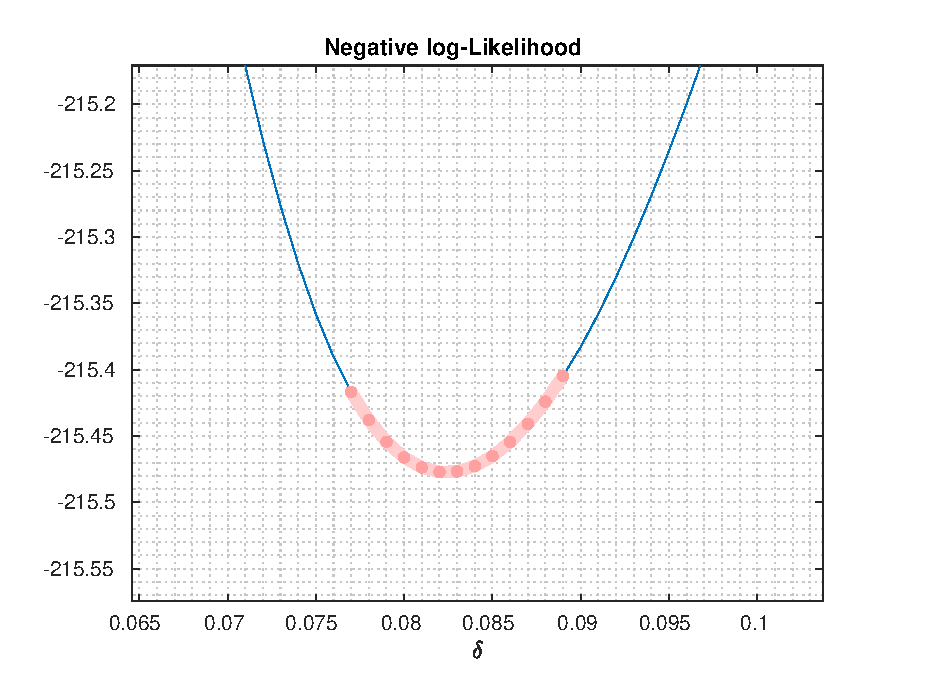
\includegraphics[width=1\textwidth]{../../MATLAB_Files/Results/delta/min.eps}

\end{columns}

\end{frame}


\setbeamercolor{background canvas}{bg=white!10}
\begin{frame}\frametitle{Step by step: Averaged $m_2(t_0)$ over all the the used samples}

\begin{figure}[ht!]
\centering
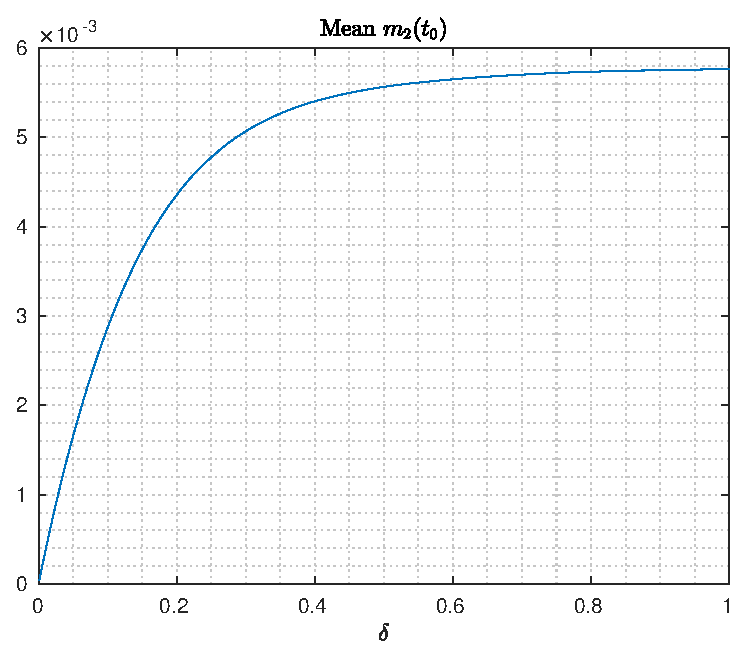
\includegraphics[width=0.45\textwidth]{../../MATLAB_Files/Results/delta/M2_0.eps}
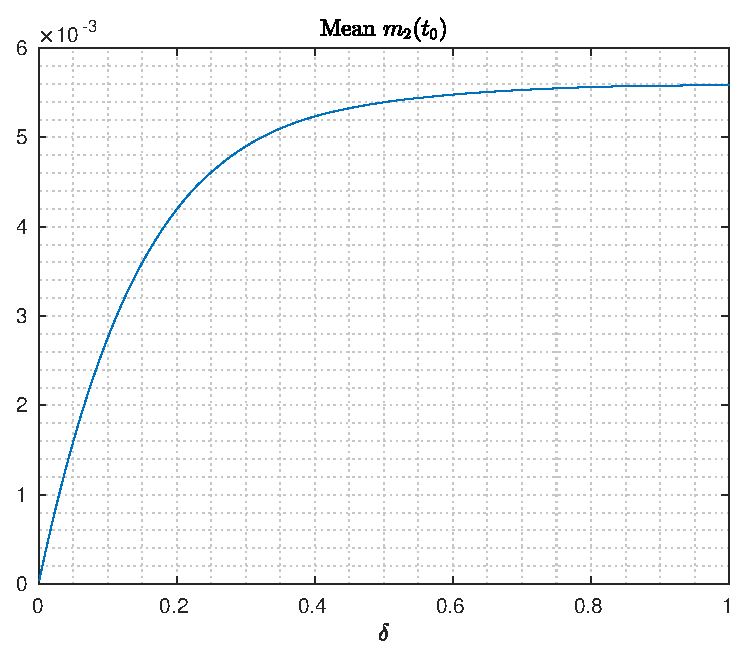
\includegraphics[width=0.45\textwidth]{../../MATLAB_Files/Results/delta/M2_1.eps}
\end{figure}
On the left, all initial points. On the right, only the {\color{orange}*corrected data* with $\eta=0.1$}.
\end{frame}


\setbeamercolor{background canvas}{bg=white!10}
\begin{frame}\frametitle{Step by step: Averaged $\sigma^2(t_0)$ over all the used samples}

\begin{figure}[ht!]
\centering
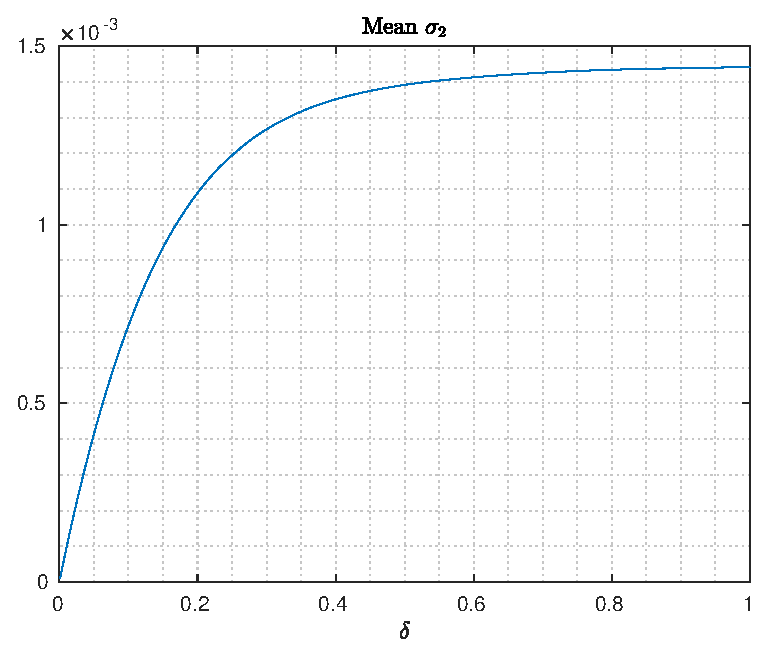
\includegraphics[width=0.45\textwidth]{../../MATLAB_Files/Results/delta/Sig_0.eps}
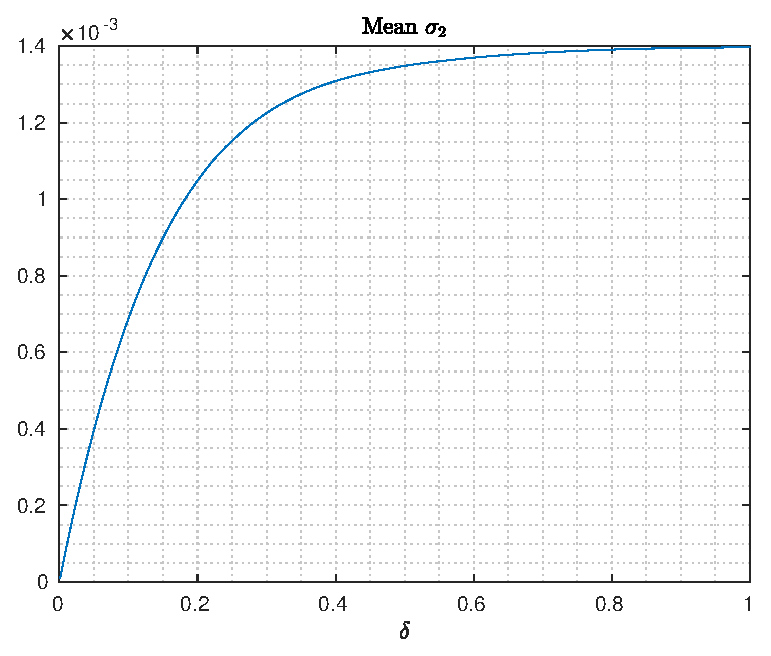
\includegraphics[width=0.45\textwidth]{../../MATLAB_Files/Results/delta/Sig_1.eps}
\end{figure}
On the left, all initial points. On the right, only the {\color{orange}*corrected data* with $\eta=0.1$}.
\end{frame}


\setbeamercolor{background canvas}{bg=white!10}
\begin{frame}\frametitle{Some remarks:}

\begin{itemize}

\item We showed plots with $\eta=0.1$. Smaller values also work, but we want to modify the data as few as possible. \alert{Can we plot $\delta$ w.r.t. $\eta$? See next slide.}
\item $1/4$ is a very large upper bound, as we assumed $p_t(1-p(t))=1/4$ for all time. This is the reason why the plots show values of variance smaller by orders of magnitude.
\item By construction of our model, if $m_1(t_0)=0$, then $\xi_1=\xi_2$. And then, $\sigma^2=m_2(t_0)$.
\item We bounded the variance using that $m_1(t)=0$. With no this assumption, maybe we can reach any value of variance.

\end{itemize}

\end{frame}


\setbeamercolor{background canvas}{bg=white!10}
\begin{frame}\frametitle{$\delta$ over $\eta$:}

\begin{figure}[ht!]
\centering
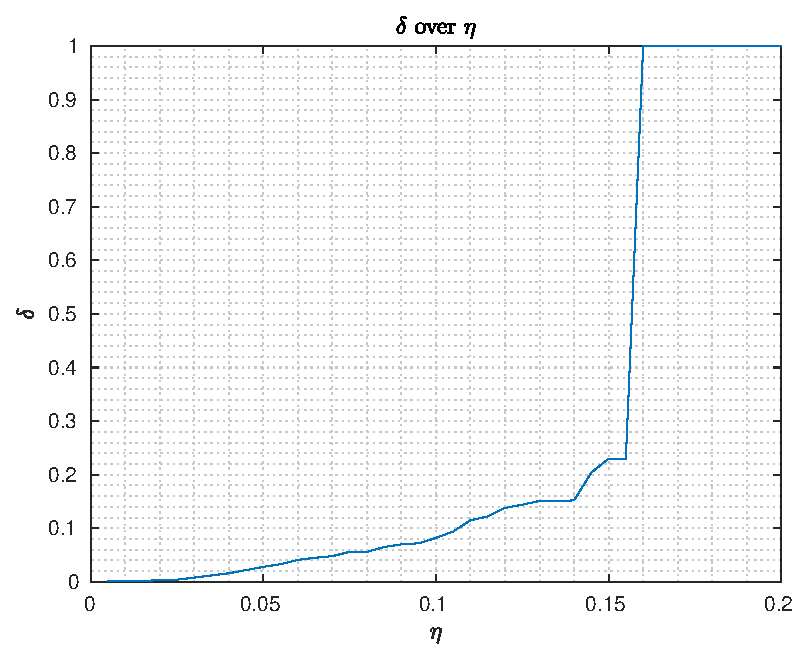
\includegraphics[width=0.45\textwidth]{../../MATLAB_Files/Results/delta/eta.eps}
\includegraphics[width=0.45\textwidth]{../../MATLAB_Files/Results/delta/eta_min.eps}
\end{figure}
{\color{orange}We choose $\eta=0.15$ which leads to $\delta=\SI{330}{\min}=\SI{5.5}{\hour}$.} \alert{However, this plot is highly dependent on $\alpha$ and $\theta_0$. Then, our selection of $\delta$ may change before and after finding the optimal parameters.}
\end{frame}


\setbeamercolor{background canvas}{bg=white!10}
\begin{frame}\frametitle{$\delta$ over $\eta$:}

\begin{figure}[ht!]
\centering
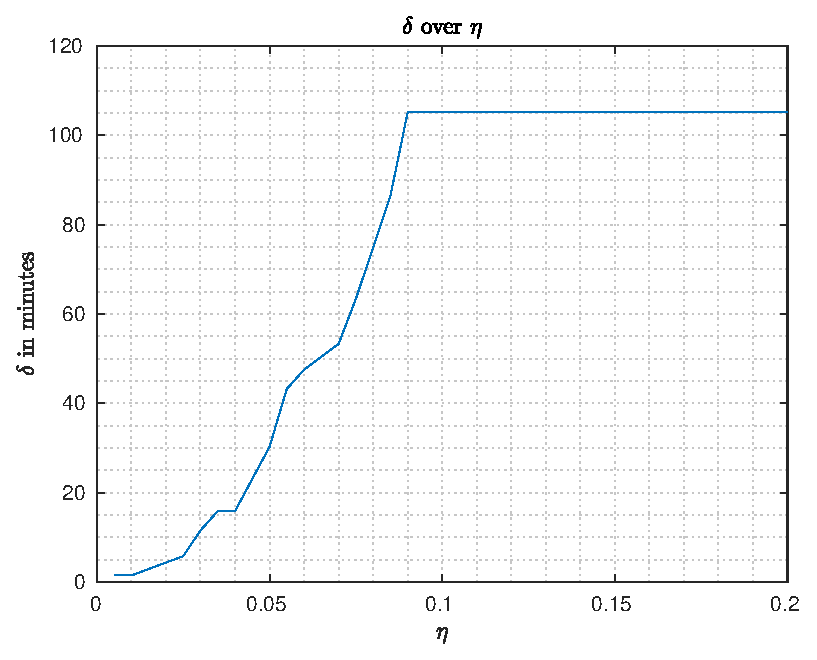
\includegraphics[width=0.4\textwidth]{../../MATLAB_Files/Results/delta/eta_min_ini.eps}\quad\quad
\includegraphics[width=0.4\textwidth]{../../MATLAB_Files/Results/delta/eta_min_opt.eps}
\end{figure}
On the left, we use the initial $(\theta_0,\alpha)$ ($\alpha\theta_0=0.1$) and we get $\delta=\SI{220}{\min}$.\\
On the right, we use the optimal ones. As the optimal product $\alpha\theta_0$ ($\alpha\theta_0=0.08$) is smaller than the initial one, we need a larger $\delta$ to match the variance of the initial error, or to remove some data. If we remove up to $\eta=0.1$, we get $\delta=\SI{220}{\min}$.
\end{frame}

\end{document}